\documentclass[12pt,fleqn]{article}\usepackage{../common}
\begin{document}
Paralel Matris �arp�m�, Ax, QR ve SVD

{\em Matris �arp�m�} adli yazi tek makinali ortamda matris carpiminin
nasil yapilacagini, ve nasil gorulecebilegini anlatti. Satir bakis
acisi, kolon bakis acisi islendi. Parallel (Hadoop), esle/indirge
ortaminda matris carpimini nasil yapariz?  Mesela $A^TA$'yi ele
alalim. Bu carpim oldukca onemli cunku baska sonuclar icin de
kullanilabiliyor. Mesela $A$ uzerinde $QR$ ayristirmasi yapmak
isterseniz (bkz. Lineer Cebir ders notlarimiz) bu carpim
kullanilabiliyor.

Nasil? QR ayristirmasi kolonlarin hepsi bilindigi gibi birbirine dik
(orthogonal) birim vektorler olan bir $Q$ matrisi ve ust ucgensel
(upper triangular) bir $R$ matrisi olusturur. Ayristirmanin $A^TA$ ile
baglantisi nedir? Eger $A$ yerine onun ayristirmasini $QR$ koyarsak,

$$
C = A^TA = (QR)^T (QR) = R^T Q^T QR
$$

Tum $Q$ vektorleri birbirine dik, ve birim vektorler ise, $Q^T Q$
birim matrisi $I$ olur. O zaman

$$
C = R^T Q^T QR = R^T R
$$

Yani

$$
C = R^TR
$$

Peki $A^TA$ hesaplayip (boylece $R^TR$'yi elde edince) onun icinden
$R$'yi nasil cekip cikartiriz? Simdi Cholesky ayristirmasi kullanmanin
zamani. Cholesky ayristirmasi (herhangi bir simetrik pozitif kesin $C$
matrisi uzerinde)

$$C = LL^T$$

olarak bilinir, yani bir matris alt ucgensel (lower triangular -ki L
harfi oradan geliyor-) $L$ matrisine ve onun devrigi olan ust ucgensel
$L^T$'nin carpimina ayristirilir. Elimizde $R^TR$ var, ve ona benzer
$LL^T$ var, $R$ bilindigi gibi ust ucgensel, $L$ alt ucgensel, $L^T$
ve $R$ birbirine esit demek ki. Yani $A^TA$ uzerinde numerik hesap
kutuphenimzin Cholesky cagrisi kullanmak bize $QR$'in $R$'sini verir.

Su anda akla su soru gelebilir: madem kutuphane cagrisi yaptik, niye
$A$ uzerinde kutuphenimizin $QR$ cagrisini kullanmiyoruz?

Cevap Buyuk Veri argumaninda sakli. Bu ortamda ugrasilan verilerde $A$
matrisi $m \times n$ boyutlarindadir, ve $m$ milyonlar, hatta
milyarlarca satir olabilir. Simdilik $m >> n$ oldugunu farzedelim,
yani $m$, $n$'den "cok, cok buyuk", yani "boyut kolonlarinin", ki $n$,
sayisi binler ya da onbinlerde. Bu gayet tipik bir senaryo aslinda,
olcum noktalari (boyutlar) var, ama cok fazla degil, diger yandan o
olcumler icin milyonlarca veri noktasi toplanmis. Tipik bir asiri
belirtilmis (overdetermined) sistem - ki en az kareler (least squares)
gibi yaklasimlarin temel aldigi sistemler bunlardir, eldeki denklem
sayisindan daha fazla olcum noktasi vardir. Bu arada en az karelerden
bahsettik, $QR$'in kullanildigi alanlardan biri en az karelerin cozumudur.

Argumana devam ediyoruz, kutuphane <code>qr</code> cagrisini $A$
uzerinde yaparsak, $m \times n$ gibi devasa bir matris uzerinde islem
yapmak gerekir. Ama $A^TA$ uzerinde islem (Cholesky) yaparsak, ki bu
carpimin boyutu $n \times m \cdot m \times n = n \times n$, yani cok
daha ufak bir matristir. $A^TA$'in islem bedeli cok ufak, birazdan
anlatacagimiz yontem sayesinde bu bedel $O(m)$.

Paralel $A^TA$

Paralel carpima gelelim. Oncelikle elimizdeki becerilere
(capabilities) bakalim. Hadoop ortami bize asiri buyuk bir dosyayi
otomatik olarak makinalara bolerek bir hesap yapilmasi gerektiginde o
hesabin her makinada, elindeki veri parcasi uzerinde yaptirilmasini
sagliyor.

$A^TA$ orneginde eldeki veri $A$, ve "cok olan" $A$'nin satirlari,
yani $m \times n$ boyutlarinda matris var ve $m$ devasa boyutlarda
(olabilir). Bir $A$ dosyasi tipik olarak soyle gozukecek:

\begin{minted}{python}
!head -5 A_matrix
\end{minted}

\begin{verbatim}
3 4 5 6
3 4 5 2
3 6 7 8
2 2 2 2
9 9 3 3
\end{verbatim}

Esle/indirgeye gelelim: Eger carpima satir bakisini hatirlarsak,

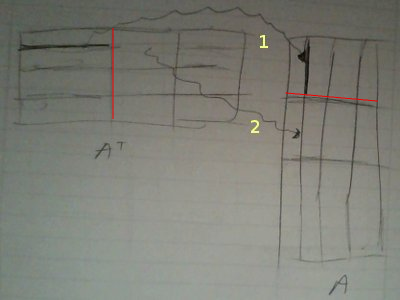
\includegraphics[height=6cm]{AtA.png}

Bu bakisa gore soldaki matriste satir boyunca giderken, sagdakinde ona
tekabul eden kolon boyunca gidiyoruz, ve birbirine eslene her ogeyi
carpiyoruz, ve carpimlari topluyoruz.

Simdi bu matrisin Hadoop'ta parca parca bize geldigini dusunursek (ki
ustte hayali bir ilk parcayi kirmizi cizgi ile belirttik), bu parca
icinde mesela ilk satiri kendisi ile carparken (1'inci ok) ayni blok
icindeyiz. Bu onemli bir nokta, carparken bloklar arasi gecis
yok.

Tabii ki nihai carpimdaki (1,1) hesabi icin $A^T$'deki birinci satirin
<i>tamamen</i> $A$'daki birinci kolonla nokta carpiminin bitirilmis
olmasi gerekir, ama simdi dusunelim, baska bir makinaya ikinci parca
verilmis ise, makinada o birinci satirin geri kalani carpilip
toplanacaktir (2. ok), ve eger tum parcalar, tum makinalarda bu
sekilde islenirse, (1,1) hesabi icin o makinalardaki o tum carpimlari
alip nihai bir noktada toplamak bize (1,1) icin nihai sonucu
verecektir. Bu tipik bir esle/indirge hesabi olabilir, esle safhasinda
eldeki parca $A_p$ uzerinde $A_p^T A_p$ yapilir, indirge safhasinda bu
parcalar toplanir.

Esleme safhasindan yayinlanacak (emit) anahtar ve degerler, bizce,
$A_p^T A_p$ icindeki her satirin satir no'su ve satir degeri
olmali. Niye? (Ayni sabit bir anahtar degeriyle beraber $A_p^T A_p$'in
tamamini da yayinlayabilirdik).

Hatirlayalim, nihai carpim $n \times n$ boyutunda, her parca $p$ olsa
bile, $n \times p \cdot p \times n$ yine bize $n \times n$
veriyor. Yani her makina $n \times n$ boyutunda bir carpim sonucunu
uretiyor. Evet $n$ nispeten kucuk bir sayi, fakat yine de onbinlerde
olsa bile $10,000 \times 10,000$ mesela, buyuk bir sayi. Eger tum
toplami tek bir indirgeyici makinaya yaptirirsak, pek cok $n \times n$
boyutunda matrisin toplami bu makinayi kasar. O sebeple indirgeme
sonrasi matrisleri degil, o matrislerin her $n$ satirini satir no'su
ile yayinliyoruz, boylece ayni satirlar ayni indirgeyiciye gidip orada
toplaniyorlar, ama bircok indirgeyici var yani toplama islemi paralel
hale gelmis oluyor. Tabii indirgeme sonrasi o sonuclar yayinlaniyor,
ve satir no'ya gore dogal olarak siralanmis halde nihai sonuc cikiyor.
Ama toplama islemi paralel. Kod alttaki gibi

\inputminted{python}{AtA.py}

Fonksiyon \verb!mapper_final! MRJob kurallarina gore bir 
makinadaki tum esleme bittikten sonra cagirilir, biz bu cengeli
(hook), "artik parcalari carpip yayinlamak icin" kullandik, her parca
$p$ buyuklugunde, ama $m / p$ tam sayi olmayabilir, yani islem sonunda
bazi artik veriler kalmis olabilir, onlari \verb!mapper_final!
icinde carpiyoruz.

Bu arada kodun kendi icinde de bir "parcalama", "biriktirme ve isleme"
yaptigina dikkat, yani 20,000 satir olabilir, iki tane esleyici var ise
her esleyici bu verinin 10,000 satirini isler, ama ayrica isleyiciler
daha ufak ufak (ustte 4) parcalarla carpim yapiyor.

\begin{minted}{python}
!python AtA.py A_matrix
\end{minted}

\begin{verbatim}
using configs in /home/burak/.mrjob.conf
creating tmp directory /tmp/AtA.burak.20131202.225802.256844
writing to /tmp/AtA.burak.20131202.225802.256844/step-0-mapper_part-00000
Counters from step 1:
  (no counters found)
writing to /tmp/AtA.burak.20131202.225802.256844/step-0-mapper-sorted
> sort /tmp/AtA.burak.20131202.225802.256844/step-0-mapper_part-00000
writing to /tmp/AtA.burak.20131202.225802.256844/step-0-reducer_part-00000
Counters from step 1:
  (no counters found)
Moving /tmp/AtA.burak.20131202.225802.256844/step-0-reducer_part-00000 -> /tmp/AtA.burak.20131202.225802.256844/output/part-00000
Streaming final output from /tmp/AtA.burak.20131202.225802.256844/output
0	"[ 420.  463.  264.  265.]"
1	"[ 463.  538.  351.  358.]"
2	"[ 264.  351.  316.  321.]"
3	"[ 265.  358.  321.  350.]"
removing tmp directory /tmp/AtA.burak.20131202.225802.256844
\end{verbatim}

Karsilastirmak icin ayni islemi tek bir script icinde yapalim, 

\begin{minted}{python}
%pylab inline
A = np.loadtxt('A_matrix')
print np.dot(A.T,A)
\end{minted}

\begin{verbatim}
[[ 420.  463.  264.  265.]
 [ 463.  538.  351.  358.]
 [ 264.  351.  316.  321.]
 [ 265.  358.  321.  350.]]
\end{verbatim}

Tipatip ayni. 

Simdi bu sonuc uzerinde Cholesky yapalim

\begin{minted}{python}
import numpy.linalg as lin
print lin.cholesky(np.dot(A.T,A))
\end{minted}

\begin{verbatim}
[[ 20.49390153   0.           0.           0.        ]
 [ 22.59208669   5.25334361   0.           0.        ]
 [ 12.88188096  11.41585875   4.44244436   0.        ]
 [ 12.93067597  12.53849977   2.54158031   4.37310096]]
\end{verbatim}

Bu bize $L$'yi verdi. Karsilastirmak icin $A$ uzerinde direk \verb!qr!
yapalim

\begin{minted}{python}
q,r = lin.qr(A)
print r.T
\end{minted}

\begin{verbatim}
[[-20.49390153   0.           0.           0.        ]
 [-22.59208669  -5.25334361   0.           0.        ]
 [-12.88188096 -11.41585875   4.44244436   0.        ]
 [-12.93067597 -12.53849977   2.54158031  -4.37310096]]
\end{verbatim}

Bu matris Cholesky sonucunun eksi ile carpilmis hali, fakat bu nihai sonuc
acisindan farketmiyor. 

Q

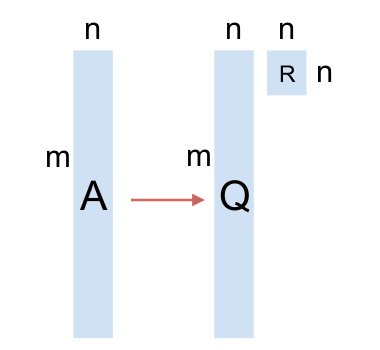
\includegraphics[height=4cm]{qr.png}

Q hesabi icin biraz daha takla atmak lazim,

$$A = QR$$

$$AR^{-1} = QRR^{-1} $$

$$Q = AR^{-1} $$

Demek ki $R$'i elde ettikten sonra onu tersine cevirip (inverse) $A$
ile carparsak, bu bize $Q$'yu verecek. Dert degil, $R$ ufak bir
matris, $n \times n$, ve tersini alma operasyonu pahali bir islem olsa
da bu boyutlarda yavas olmaz. Daha sonra bu $R^{-1}$'i alip bu sefer
baska bir esle/indirge ile carpim islemine tabi tutariz. R'yi direk
alttaki script icine yazdik (B olarak) bir sonuc ortaminda bu verinin
baska bir sekilde MRJob islemine verilmis olmasi lazim. Bir isleme
zinciri var, zincirde once $A^TA$, Cholesky, oradan $R$ alinip baska
bir isleme (job) aktariliyor. 

\inputminted{python}{AB.py}

\begin{minted}{python}
!python AB.py A_matrix
\end{minted}

\begin{verbatim}
using configs in /home/burak/.mrjob.conf
creating tmp directory /tmp/AB.burak.20131202.230008.985111
writing to /tmp/AB.burak.20131202.230008.985111/step-0-mapper_part-00000
Counters from step 1:
  (no counters found)
writing to /tmp/AB.burak.20131202.230008.985111/step-0-mapper-sorted
> sort /tmp/AB.burak.20131202.230008.985111/step-0-mapper_part-00000
writing to /tmp/AB.burak.20131202.230008.985111/step-0-reducer_part-00000
Counters from step 1:
  (no counters found)
Moving /tmp/AB.burak.20131202.230008.985111/step-0-reducer_part-00000 -> /tmp/AB.burak.20131202.230008.985111/output/part-00000
Streaming final output from /tmp/AB.burak.20131202.230008.985111/output
null	"[[ -61.48170459  -88.78963451  -62.09685608  -84.98432736]\n [ -20.49390153  -27.8454303   -19.85529535  -27.30069639]\n [ -40.98780306  -55.6908606   -39.7105907   -54.60139278]\n [-184.44511377 -250.6088727  -205.35232431 -234.71714361]]"
null	"[[ -61.48170459  -99.29632173  -76.04368486 -131.21677204]\n [ -40.98780306  -55.6908606   -39.7105907   -54.60139278]\n [-184.44511377 -250.6088727  -205.35232431 -234.71714361]\n [ -61.48170459  -88.78963451  -62.09685608 -102.4767312 ]]"
null	"[[-184.44511377 -250.6088727  -205.35232431 -234.71714361]\n [ -61.48170459  -99.29632173  -76.04368486 -131.21677204]\n [ -40.98780306  -55.6908606   -39.7105907   -54.60139278]\n [-184.44511377 -250.6088727  -205.35232431 -234.71714361]]"
null	"[[ -61.48170459  -88.78963451  -62.09685608 -102.4767312 ]\n [ -61.48170459  -88.78963451  -62.09685608  -84.98432736]\n [ -61.48170459  -99.29632173  -76.04368486 -131.21677204]\n [ -40.98780306  -55.6908606   -39.7105907   -54.60139278]]"
removing tmp directory /tmp/AB.burak.20131202.230008.985111
\end{verbatim}

Kontrol edelim,

\begin{minted}{python}
B = np.array([[-20.49390153,   0.        ,   0.        ,   0.        ],
              [-22.59208669,  -5.25334361,   0.        ,   0.        ],
              [-12.88188096, -11.41585875,   4.44244436,   0.        ],
              [-12.93067597, -12.53849977,   2.54158031,  -4.37310096]])
print np.dot(A,B.T)
\end{minted}

\begin{verbatim}
[[ -61.48170459  -88.78963451  -62.09685608 -102.4767312 ]
 [ -61.48170459  -88.78963451  -62.09685608  -84.98432736]
 [ -61.48170459  -99.29632173  -76.04368486 -131.21677204]
 [ -40.98780306  -55.6908606   -39.7105907   -54.60139278]
 [-184.44511377 -250.6088727  -205.35232431 -234.71714361]
 [ -61.48170459  -99.29632173  -76.04368486 -131.21677204]
 [ -40.98780306  -55.6908606   -39.7105907   -54.60139278]
 [-184.44511377 -250.6088727  -205.35232431 -234.71714361]
 [ -61.48170459  -99.29632173  -76.04368486 -131.21677204]
 [ -40.98780306  -55.6908606   -39.7105907   -54.60139278]
 [-184.44511377 -250.6088727  -205.35232431 -234.71714361]
 [ -61.48170459  -88.78963451  -62.09685608 -102.4767312 ]
 [ -61.48170459  -88.78963451  -62.09685608  -84.98432736]
 [ -20.49390153  -27.8454303   -19.85529535  -27.30069639]
 [ -40.98780306  -55.6908606   -39.7105907   -54.60139278]
 [-184.44511377 -250.6088727  -205.35232431 -234.71714361]
 [ -81.97560612 -116.63506481  -90.83704015 -126.11438629]]
\end{verbatim}

Carpimlar ayni. Yanliz dikkat, satirlarin sirasi degisik olabilir,
burada problem esle/indirge isleminin $A$'yi parcalama sonucu her
carpim parcasinin degisik bir sirada ele geciyor olmasi. Eger
siralamayi ayni $A$ gibi istiyorsak, bu sira no'sunu $A$ verisi icinde
ilk satira koymak lazim ve esleyiciler oradan alip bu no'yu anahtar
olarak yayinlamalilar. Bu eklemeyi okuyucuya birakiyorum!

Simdi QR hesabini bu sekilde yapip yapamayacagimizi kontrol
edelim. Eger \verb!qr! ile $Q$ hesaplarsak,

\begin{minted}{python}
q,r = lin.qr(A)
print q
\end{minted}

\begin{verbatim}
[[-0.14638501 -0.13188879  0.36211188 -0.35057934]
 [-0.14638501 -0.13188879  0.36211188  0.56410341]
 [-0.14638501 -0.51259871 -0.16600517 -0.02328772]
 [-0.09759001  0.03897744  0.26737941 -0.1251395 ]
 [-0.43915503  0.1753985  -0.14740047  0.02394349]
 [-0.14638501 -0.51259871 -0.16600517 -0.02328772]
 [-0.09759001  0.03897744  0.26737941 -0.1251395 ]
 [-0.43915503  0.1753985  -0.14740047  0.02394349]
 [-0.14638501 -0.51259871 -0.16600517 -0.02328772]
 [-0.09759001  0.03897744  0.26737941 -0.1251395 ]
 [-0.43915503  0.1753985  -0.14740047  0.02394349]
 [-0.14638501 -0.13188879  0.36211188 -0.35057934]
 [-0.14638501 -0.13188879  0.36211188  0.56410341]
 [-0.048795    0.01948872  0.1336897  -0.06256975]
 [-0.09759001  0.03897744  0.26737941 -0.1251395 ]
 [-0.43915503  0.1753985  -0.14740047  0.02394349]
 [-0.19518001 -0.11240007  0.04559899 -0.21745867]]
\end{verbatim}

$R$'in tersi ile $A$ carpilinca hakikaten $Q$ elde ediliyor mu?
Kontrol edelim.

\begin{minted}{python}
print np.dot(A,lin.inv(B.T))
\end{minted}

\begin{verbatim}
[[-0.14638501 -0.13188879  0.36211188 -0.35057934]
 [-0.14638501 -0.13188879  0.36211188  0.56410341]
 [-0.14638501 -0.51259871 -0.16600517 -0.02328772]
 [-0.09759001  0.03897744  0.26737941 -0.1251395 ]
 [-0.43915503  0.1753985  -0.14740047  0.02394349]
 [-0.14638501 -0.51259871 -0.16600517 -0.02328772]
 [-0.09759001  0.03897744  0.26737941 -0.1251395 ]
 [-0.43915503  0.1753985  -0.14740047  0.02394349]
 [-0.14638501 -0.51259871 -0.16600517 -0.02328772]
 [-0.09759001  0.03897744  0.26737941 -0.1251395 ]
 [-0.43915503  0.1753985  -0.14740047  0.02394349]
 [-0.14638501 -0.13188879  0.36211188 -0.35057934]
 [-0.14638501 -0.13188879  0.36211188  0.56410341]
 [-0.048795    0.01948872  0.1336897  -0.06256975]
 [-0.09759001  0.03897744  0.26737941 -0.1251395 ]
 [-0.43915503  0.1753985  -0.14740047  0.02394349]
 [-0.19518001 -0.11240007  0.04559899 -0.21745867]]
\end{verbatim}

Sonuclar birebir ayni.

Ustteki teknikleri kullanarak artik devasa boyutlarda satiri olan bir
$A$ matrisi uzerinde artik QR hesabi yapabilirsiniz. 

SVD
Peki $QR$ sonuclarini kullanarak SVD sonuclarini alabilir miyiz?
SVD bize ne verir? 

$$ A = U \Sigma V^T $$

$U$ ve $V^T$ ortogonal matrislerdir, $\Sigma$ sadece kosegeni boyunca
degerleri olan bir matristir. Daha fazla detay icin <i>Lineer Cebir
Ders 29</i>'a bakabilirsiniz. Simdi $A = QR$ yerine koyalim,

$$ QR =  U \Sigma V^T $$

$$ R = Q^T U \Sigma V^T $$

Bu son formuled $Q^TU$ formulu, iki ortogonal matrisin carpimidir. Lineer
Cebir kurallarina gore iki ortogonal matrisin carpimi bir diger ortogonal
matristir. Bu yeni ortogonal matrise $U_R$ adi verelim, o zaman

$$ R = U_R \Sigma V^T $$

Bu son formul bize bir seyler soyluyor. $R$'nin SVD uzerinden
ayristirilabilecegini soyluyor ve bu ayristirma sonrasi ele gecen
$U_R,V^T$ ve $\Sigma$ kosegen matrisleridir! Bu cok onemli bir sonuc.
Bu ayristirmanin sonucu $A$'nin ki ile birbirine cok benziyor, tek
fark $U$ ile $U_R$. Bu iki matris arasindaki gecis soyle:

$$ U_R = Q^T U $$ 

$$ U = QU_R $$ 

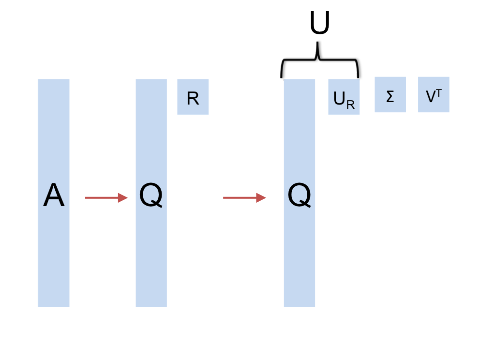
\includegraphics[height=6cm]{ur.png}

Bu demektir ki eger $R$ uzerinde kutuphanemizin \verb!svd!
cagrisini kullanirsak (ki $R$ nispeten ufak oldugu icin bu ucuz olur)
ele gecen $U_R$'i alip, $Q$ ile carparsak, $A$ ayristirmasinin
$U$'sunu elde ederiz! $Q$ ile carpim esle/indirge uzerinden
yapilabilir, fakat basit bir carpim islemi oldugu icin paralelize
edilmesi kolaydir (ustteki mrjob script'inde yaptigimiz gibi).

Kaynaklar

[1] Benson, A., Tall-and-skinny Matrix Computations in MapReduce

[2] Constantine, P. G., Gleich, D. F. , Tall and Skinny QR factorizations
in MapReduce architectures

[3] Dasgupta, S., Gupta, A., An Elementary Proof of a Theorem of Johnson
and Lindenstrauss














\end{document}
